% !TeX program = xelatex
\documentclass[12pt,a4paper,oneside]{book}

\usepackage{iftex}
\ifXeTeX
  \usepackage{fontspec}
  \usepackage{polyglossia}
  \setdefaultlanguage{english}
  \setotherlanguage{french}
  \setotherlanguage{arabic}
  \makeatletter
  \nofrench@punctuation
  \makeatother
  \setmainfont{TeX Gyre Pagella}
  \setsansfont{TeX Gyre Heros}
  \setmonofont{TeX Gyre Cursor}
  \IfFontExistsTF{Amiri}{%
    \newfontfamily\arabicfont[Script=Arabic,Scale=1.06]{Amiri}%
  }{%
    \IfFontExistsTF{Noto Naskh Arabic}{%
      \newfontfamily\arabicfont[Script=Arabic,Scale=1.06]{Noto Naskh Arabic}%
    }{%
      \newfontfamily\arabicfont[Script=Arabic,Scale=1.06]{Arabic Typesetting}%
    }%
  }%
  \providecommand{\textarabic}[1]{\foreignlanguage{arabic}{#1}}%
\else
  \usepackage[T1]{fontenc}
  \usepackage[utf8]{inputenc}
  \usepackage[french,english]{babel}
  \usepackage{tgpagella}
  \newcommand{\textenglish}[1]{#1}%
  \newcommand{\textarabic}[1]{#1}%
  \newenvironment{Arabic}{}{}%
\fi
\usepackage{geometry}
\usepackage{graphicx}
\usepackage{grffile}
\graphicspath{{Figures/}{Logos/}{images/}{diagrams/}{Screenshots/}}
% svg package removed: Overleaf/pdflatex uses PNG/PDF figures only (no shell-escape)
\usepackage{float}
\usepackage{placeins}
\usepackage{booktabs}
\usepackage{longtable}
\usepackage{tabularx}
\usepackage{array}
\usepackage{amsmath}
\usepackage{amssymb}
\usepackage{setspace}
\usepackage{xcolor}
\usepackage{colortbl}
\definecolor{navyblue}{RGB}{20,55,95}
\usepackage{enumitem}
\usepackage{mdframed}
\PassOptionsToPackage{hyperfootnotes=false}{hyperref}
\usepackage{hyperref}
\usepackage{titlesec}
\usepackage{fancyhdr}
\usepackage{listings}
\usepackage{caption}
\usepackage{microtype}
\usepackage{silence}
\WarningFilter{tracklang}{No `datatool' support for dialect}
\WarningFilter{latex}{Infinite glue shrinkage found in box being split}
\usepackage{afterpage}
\usepackage{pdfpages}
\usepackage[acronym]{glossaries}

\geometry{
    a4paper,
    left=2.5cm,
    right=2.5cm,
    top=2.6cm,
    bottom=2.6cm
}

\setlength{\headheight}{16pt}
\pagestyle{fancy}
\fancyhf{}
\fancyhead[L]{\nouppercase{\leftmark}}
\fancyhead[R]{\thepage}
\renewcommand{\headrulewidth}{0.3pt}
\renewcommand{\footrulewidth}{0pt}

\renewcommand{\chaptermark}[1]{\markboth{\MakeUppercase{#1}}{}}
\renewcommand{\sectionmark}[1]{\markright{\thesection.\ #1}}

\onehalfspacing
\setlength{\parindent}{1.5em}
\setlength{\parskip}{0.12\baselineskip plus 0.04\baselineskip minus 0.04\baselineskip}
\setcounter{secnumdepth}{3}
\setcounter{tocdepth}{3}
\setlength{\emergencystretch}{3em}
\hbadness=10000
\hfuzz=1pt
\setlength{\tabcolsep}{4.5pt}
\setlength{\LTleft}{0pt}
\setlength{\LTright}{0pt}
\setlength{\LTcapwidth}{\textwidth}
\renewcommand{\tabularxcolumn}[1]{>{\raggedright\arraybackslash}m{#1}}

\newcolumntype{Y}{>{\raggedright\arraybackslash}X}
\newcolumntype{P}[1]{>{\raggedright\arraybackslash}p{#1}}

\definecolor{codegreen}{rgb}{0,0.5,0}
\definecolor{codegray}{rgb}{0.45,0.45,0.45}
\definecolor{codepurple}{rgb}{0.58,0,0.82}
\definecolor{backcolour}{rgb}{0.97,0.97,0.95}

\lstdefinestyle{mystyle}{
    backgroundcolor=\color{backcolour},
    commentstyle=\color{codegreen},
    keywordstyle=\color{magenta},
    numberstyle=\tiny\color{codegray},
    stringstyle=\color{codepurple},
    basicstyle=\ttfamily\footnotesize,
    breakatwhitespace=false,
    breaklines=true,
    captionpos=b,
    keepspaces=true,
    numbers=left,
    numbersep=6pt,
    showspaces=false,
    showstringspaces=false,
    showtabs=false,
    tabsize=2
}

\lstset{style=mystyle}
\renewcommand{\lstlistingname}{Code Listing}
\renewcommand{\lstlistlistingname}{List of Code Listings}

\definecolor{primary}{HTML}{1A237E}
\definecolor{accent}{HTML}{0277BD}
\definecolor{success}{HTML}{2E7D32}
\definecolor{warning}{HTML}{BF360C}
\definecolor{lightblue}{HTML}{E3F2FD}
\definecolor{lightgreen}{HTML}{E8F5E9}
\definecolor{lightyellow}{HTML}{FFFDE7}
\definecolor{subtle}{HTML}{546E7A}

\newmdenv[backgroundcolor=lightblue,linecolor=accent,linewidth=1.5pt,
  leftline=true,topline=false,rightline=false,bottomline=false,
  innerleftmargin=10pt,innerrightmargin=8pt,innertopmargin=7pt,innerbottommargin=7pt,
  skipabove=8pt,skipbelow=8pt]{infobox}
\newmdenv[backgroundcolor=lightgreen,linecolor=success,linewidth=1.5pt,
  leftline=true,topline=false,rightline=false,bottomline=false,
  innerleftmargin=10pt,innerrightmargin=8pt,innertopmargin=7pt,innerbottommargin=7pt,
  skipabove=8pt,skipbelow=8pt]{successbox}
\newmdenv[backgroundcolor=lightyellow,linecolor=warning,linewidth=1.2pt,
  leftline=true,topline=false,rightline=false,bottomline=false,
  innerleftmargin=10pt,innerrightmargin=8pt,innertopmargin=7pt,innerbottommargin=7pt,
  skipabove=8pt,skipbelow=8pt]{riskbox}

\newcommand{\reportchapter}[3]{%
  \chapter{#2}%
  \vspace{-0.2cm}
  \begin{center}
    {\small\itshape\color{subtle}#3}
  \end{center}
  \vspace{0.25cm}
}

\newenvironment{dedication}
  {
   \clearpage
   \thispagestyle{empty}
   \vspace*{\stretch{1}}
   \begin{center}
   {\Huge\bfseries Dedication\par}
   \vspace{1cm}
   \itshape
   \begin{minipage}{1\textwidth}
   \raggedright
  }
  {
   \end{minipage}
   \end{center}
   \vspace{\stretch{2}}
   \clearpage
  }
\newcommand\blankpage{%
    \null
    \thispagestyle{empty}%
    \addtocounter{page}{-1}%
    \newpage
}

\hypersetup{colorlinks=true,linkcolor=navyblue,citecolor=navyblue,urlcolor=navyblue,
  pdfauthor={Fatima Ezzahrae Fadel; Wijdane El Hariri},pdftitle={Moroccan GraphRAG Platform},pdfpagemode=UseOutlines}

\begin{document}
\hypersetup{pageanchor=false}
\thispagestyle{empty}
\noindent
\begin{minipage}[c]{0.30\textwidth}
  
\includegraphics[height=1.9cm]{Logos/Logo_INPT.png}
\end{minipage}\hfill
\begin{minipage}[c]{0.30\textwidth}\raggedleft
  
\includegraphics[height=1.9cm]{Logos/ANRT_logo.png}
\end{minipage}
\vspace{0.9cm}
\begin{center}
{\large\textsc{\textbf{Technical Report}}}\\[0.12cm]
{\normalsize\textsc{Module: Big Data Analytics / Major: Innovation and AMOA}}\\[0.35cm]
\rule{\linewidth}{0.3mm}\\[0.3cm]
{\Large\bfseries Moroccan Business Intelligence Graph: A GraphRAG Platform for Arabic/French Sources}\\[0.15cm]
\rule{\linewidth}{0.3mm}\\[0.8cm]
\vspace{0.35cm}
\begin{minipage}{0.9\textwidth}\raggedright
\emph{Prepared by:}\\
\textsc{Fatima Ezzahrae Fadel}\\
\textsc{Wijdane El Hariri}
\end{minipage}\\[0.65cm]
{\normalsize\textit{Under the supervision of}}\\[0.15cm]
{\large\textsc{Hamid El Ghazi}}\\[0.35cm]
\vfill

\includegraphics[width=0.48\linewidth]{Logos/ANRT_logo.png}\\[0.12cm]
{\normalsize\textsc{Agence Nationale de R\'eglementation des T\'el\'ecommunications}}\\[0.08cm]
{\normalsize 2026}
\end{center}

\afterpage{\blankpage}
\frontmatter
\pagenumbering{arabic}
\chapter*{Abstract}
\addcontentsline{toc}{chapter}{Abstract}
\begingroup\setstretch{1.08}
This report presents a Graph Retrieval-Augmented Generation (GraphRAG) platform for Moroccan business intelligence. The system crawls explicitly authorised Arabic, French and English sources, extracts HTML, RSS and PDF content with provenance, stores a raw zone in HDFS when available, and applies Spark-backed ETL before indexing documents and chunks. Mistral is used for entity and relation extraction, while NVIDIA embeddings support semantic retrieval. A FastAPI service exposes graph analytics, source exploration and grounded conversational answers, and a React frontend provides operational, source and evaluation views. The validation combines retrieval metrics with Ragas faithfulness, answer relevance and context-precision measurements, while clearly distinguishing smoke evaluation from independently reviewed test cases.

\par\medskip
\noindent\rule{\textwidth}{0.5pt}\par\smallskip
{\textbf{Keywords:}} GraphRAG, Moroccan business intelligence, Scrapy, PDF extraction, Mistral, NVIDIA embeddings, HDFS, Spark, FastAPI, Ragas.\par\smallskip
\noindent\rule{\textwidth}{0.5pt}
\endgroup

\tableofcontents
\addcontentsline{toc}{chapter}{Table of Contents}
\mainmatter
\hypersetup{pageanchor=true}
\chapter*{General Introduction}
\addcontentsline{toc}{chapter}{General Introduction}

Moroccan economic information is distributed across institutional websites, reports, RSS feeds and PDF publications. Analysts need answers that are fast to explore but also traceable to an original source. This report presents a Graph Retrieval-Augmented Generation (GraphRAG) platform prepared for \textbf{l'Agence Nationale de Réglementation des Télécommunications (ANRT)}.

The objective is to combine respectful crawling, PDF and web extraction, multilingual processing, a knowledge graph, vector retrieval and a grounded chat assistant. The platform also exposes source provenance, pipeline status and evaluation statistics through a FastAPI backend and a React frontend.

The report first presents the architecture, then explains each principal pipeline component, before introducing Ragas and presenting the evaluation statistics and results. It closes with the main conclusions and perspectives.

\chapter{Architecture}
\label{chap:architecture}

\section{Overview}
The platform follows a layered architecture. The ingestion layer collects explicitly authorised sources. The processing layer validates, normalizes and chunks documents. The intelligence layer extracts entities and relations with Mistral and creates NVIDIA embeddings. The storage layer combines a raw zone, a graph store and a vector index. Finally, FastAPI exposes the services to a React interface.

\begin{figure}[H]
\centering
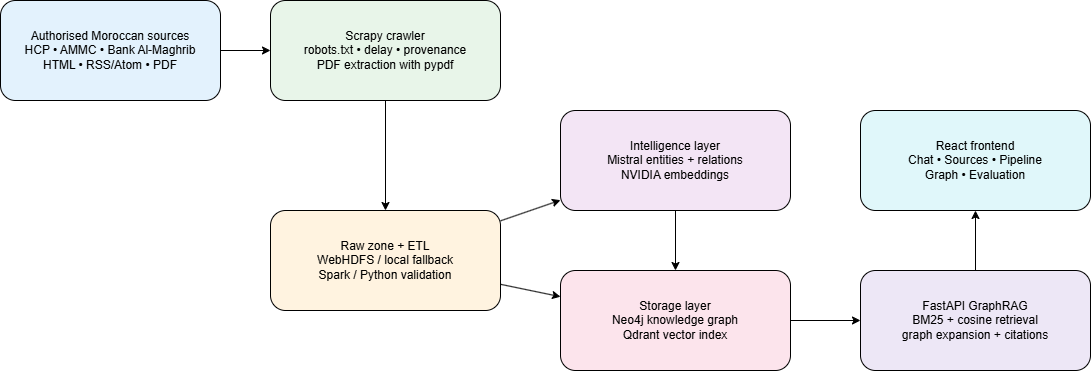
\includegraphics[width=\textwidth]{images/00-general-architecture.png}
\caption{General architecture of the Moroccan GraphRAG platform.}
\label{fig:general-architecture}
\end{figure}

\section{Information Flow}
The flow is: source URL $\rightarrow$ Scrapy item $\rightarrow$ raw document $\rightarrow$ Spark/Python ETL $\rightarrow$ chunks $\rightarrow$ graph and vector indexes $\rightarrow$ GraphRAG retrieval $\rightarrow$ cited answer. Each page keeps its URL, domain, title, language, document type and crawl timestamp.

\section{Deployment}
Docker Compose runs the API, frontend, ingestion worker, Qdrant and Neo4j. WebHDFS and Spark are optional integrations with local fallbacks for development. This keeps the prototype executable on a workstation while preserving a path to distributed deployment.

\begin{figure}[H]
\centering
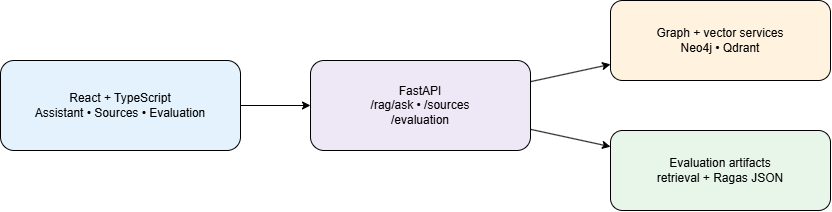
\includegraphics[width=0.9\textwidth]{images/06-frontend-compose.png}
\caption{Frontend, API and service deployment view.}
\label{fig:deployment}
\end{figure}

\section{Current Corpus and Target Sources}
The current indexed corpus contains \textbf{48 documents}: 35 HTML pages, 10 RSS/Atom entries and 3 PDF documents. The documents come from three domains: HCP (24), AMMC (16) and Bank Al-Maghrib (8). The configured targets are the HCP enterprise and economy pages, the AMMC issuer financial-statements page, Bank Al-Maghrib statistics, the Bank Al-Maghrib annual report PDF and the HCP RSS feed.

\chapter{Principal Pipeline Components}
\label{chap:pipeline}

\section{Crawler and PDF Sources}
Scrapy crawls only configured and authorised targets, obeys robots.txt and uses conservative delays. HTML pages, RSS/Atom feeds and PDFs are dispatched through the same provenance-aware parser. PDF text is extracted with \texttt{pypdf}; short or failed extractions are rejected or recorded as failures.

\begin{figure}[H]
\centering
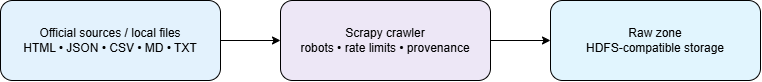
\includegraphics[width=0.9\textwidth]{images/01-ingestion.png}
\caption{Source ingestion and crawler flow.}
\label{fig:ingestion}
\end{figure}

\section{Raw Storage and ETL}
The raw zone writes to WebHDFS when enabled and falls back to local storage when the namenode is unavailable. Spark performs deduplication, whitespace normalization, source-domain normalization and minimum-text validation. A pure-Python ETL path remains available for local testing.

\begin{figure}[H]
\centering
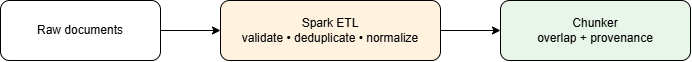
\includegraphics[width=0.9\textwidth]{images/02-etl-chunking.png}
\caption{ETL, validation and chunking stages.}
\label{fig:etl-chunking}
\end{figure}

\section{Chunking and Embeddings}
Validated pages are divided into overlapping text chunks using an 800-character window and 120-character overlap. The resulting step is 680 characters, which preserves context across boundaries. NVIDIA's embedding model \texttt{nvidia/nemotron-3-embed-1b} indexes the chunks in Qdrant. The offline deterministic test fallback uses 256 dimensions; production Qdrant collections take the dimension returned by the NVIDIA endpoint.

\section{BM25 and Hybrid Retrieval}
Retrieval combines cosine similarity from embeddings with BM25 lexical relevance. BM25 uses $k_1=1.2$, $b=0.75$ and a lexical multiplier of 2.2, with inverse document frequency computed over the indexed chunks and document-length normalization against the average chunk length. This hybrid score helps preserve exact names, acronyms and French/Arabic terms that may be missed by semantic similarity alone.

\section{Entity and Relation Extraction}
Mistral is used to extract typed entities and relations from chunks. The graph stores provenance through page and chunk links. A heuristic fallback, durable retry queue and extraction cache make failures visible without silently losing records.

\begin{figure}[H]
\centering
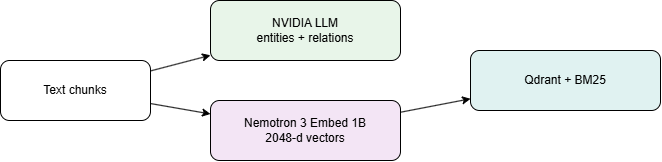
\includegraphics[width=0.9\textwidth]{images/03-extraction-embeddings.png}
\caption{Entity extraction and embedding generation.}
\label{fig:extraction-embeddings}
\end{figure}

\section{GraphRAG API and Frontend}
FastAPI exposes grounded questions, graph analytics, source pagination, PDF viewing, pipeline status and evaluation statistics. The React frontend provides the assistant conversation, source pages, graph explorer, operational pipeline view and evaluation dashboard.

\begin{figure}[H]
\centering
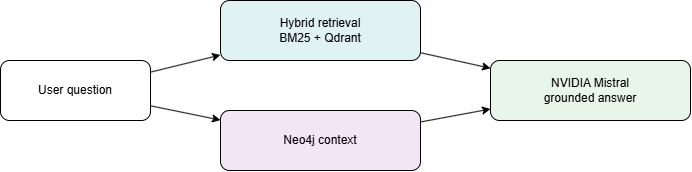
\includegraphics[width=0.9\textwidth]{images/05-graphrag-api.png}
\caption{GraphRAG API and retrieval flow.}
\label{fig:graphrag-api}
\end{figure}

\chapter{Evaluation}
\label{chap:evaluation}

\section{What is Ragas?}
Ragas is an evaluation framework for retrieval-augmented generation. It measures the quality of generated answers against their retrieved context. In this project, the principal metrics are faithfulness, answer relevancy and context precision. Faithfulness checks whether the answer is supported by the context; answer relevancy checks whether it addresses the question; and context precision checks whether the retrieved passages are useful and well-ranked.

\section{Retrieval Evaluation}
The current reviewed evaluation contains 39 documents, 534 chunks and 4 questions. Vector retrieval and GraphRAG both achieved Recall@5 of 0.75, MRR of 0.5833 and nDCG@5 of 0.625. Mean latency was 74.36 ms for vector retrieval and 94.32 ms for GraphRAG. The result is a tie: on this small corpus, the graph contributes explainability and provenance rather than a measured ranking advantage.

\begin{figure}[H]
\centering
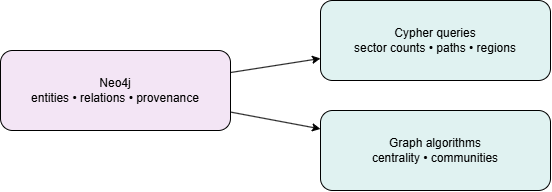
\includegraphics[width=0.9\textwidth]{images/04-neo4j-analytics.png}
\caption{Knowledge-graph storage and analytics view.}
\label{fig:graph-analytics}
\end{figure}

\section{Ragas Results}
Ragas execution is wired through \texttt{scripts/evaluate\_ragas.py} and its results are exposed by the FastAPI \texttt{/evaluation} endpoint. The frontend displays faithfulness, answer relevancy and context precision when \texttt{data/ragas\_results.json} is available. Scores must be generated with valid provider credentials; missing scores are not presented as successful results.

\section{Data Quality Statistics}
The source-quality checker currently reports an average score of \textbf{76.6/100}. It combines authority, provenance, completeness and freshness. The corpus is therefore suitable for a functional demonstration, but the score is a provenance heuristic rather than a human-annotated truth-quality measure.

\section{Interpretation and Limits}
The retrieval cases are reviewed external cases, but the corpus remains small. Ragas scores should therefore be interpreted as an initial quality signal, not as a generalization guarantee. A larger reviewed Arabic/French question set and repeated provider-controlled runs are required for a final benchmark.

\chapter*{Conclusion and Perspectives}
\addcontentsline{toc}{chapter}{Conclusion and Perspectives}

This report presented a Moroccan GraphRAG platform for source-grounded business intelligence at ANRT. The solution connects respectful HTML, RSS and PDF crawling with Spark/HDFS-ready ingestion, Mistral extraction, NVIDIA embeddings, graph and vector storage, FastAPI services and a React interface.

The platform was validated through automated tests, source-quality scoring, retrieval metrics and a Ragas execution path. The current retrieval benchmark reports a 0.75 Recall@5 tie between vector and GraphRAG retrieval, confirming a functional baseline while highlighting the need for a larger reviewed evaluation set.

Future work includes adding an HDFS namenode and Spark cluster to the deployment, running Ragas with a curated multilingual dataset, adding authentication and authorization, and measuring extraction quality separately from retrieval quality.

\end{document}
